\documentclass[a4paper,12pt]{article}
\usepackage{amsmath,amssymb,amsfonts,amsthm}
\usepackage{tikz}
\usepackage [utf8x] {inputenc}
\usepackage [T2A] {fontenc} 
\usepackage[russian]{babel}
\usepackage{cmap}
\usepackage{amsmath,amsfonts,amssymb,amsthm,mathtools} % AMS
\usepackage{graphicx}
\usepackage{wrapfig}
\usepackage{gensymb}
\usepackage{textcomp}
\usepackage{indentfirst}
\usepackage{floatrow}
\usepackage{multirow}
\usepackage{multicol} % Несколько колонок
\usepackage[version=3]{mhchem}
% вы сможете вставлять картинки командой \includegraphics[width=0.7\textwidth]{ИМЯ ФАЙЛА}
% получается подключать, как минимум, файлы .pdf, .jpg, .png.
\usepackage{mathtext} 				% русские буквы в фомулах
% Если вы хотите явно указать поля:
\usepackage[margin=1in]{geometry}
% Или если вы хотите задать поля менее явно (чем больше DIV, тем больше места под текст):
% \usepackage[DIV=10]{typearea}

\usepackage{fancyhdr}
\pagestyle{fancy}
\makeatletter % сделать "@" "буквой", а не "спецсимволом" - можно использовать "служебные" команды, содержащие @ в названии
\fancyhead[L]{\footnotesize Основы современной физики}%Это будет написано вверху страницы слева
\fancyhead[R]{\footnotesize ФЭФМ МФТИ}
\fancyfoot[R]{\thepage}%номер страницы —- внизу справа
\fancyfoot[C]{}%по центру внизу страницы пусто

\renewcommand{\maketitle}{%
	\noindent{\bfseries\scshape\large\@title\ \mdseries\upshape}\par
	\noindent {\large\itshape\@author}
	\vskip 2ex}
\makeatother
\def\dd#1#2{\frac{\partial#1}{\partial#2}}

\title{6.11.5 Туннельный диод.}
\author{Богатова Екатерина} 
\date{\today}

\begin{document}
\maketitle
\textbf{Цель работы:} исследовать принцип действия туннельного диода, измерить его вольт-амперную характеристику и основные параметры.

\section{Теоретическое введение}
	
Туннельным диодом называется сильно легированный полупроводник, уровень Ферми которого лежит в разрешенной зоне и становятся возможны туннельные переходы электронов в области узкого $(p-n)$-перехода. 
	
Будем считать, что все состояния, лежащие ниже уровня Ферми, заполнены электроны, а выше --- свободны. Энергетические диаграммы идеального туннельного диода и его вольт-амперная характеристика показаны на рисунке \ref{pic:diode}. $\mu_n$ и $\mu_p$ обозначены уровни Ферми в $n$- и $p$-области соответственно; $E_c$ и $E_v$ - границы зоны проводимости и валентной зоны. В отсутсвии внешнего поля уровни Ферми $\mu_n$ и $\mu_p$ лежат на одной горизонтали; число дырок и электронов, туннелирующих в обе стороны, одинаково, и ток отсутствует (рисунок \ref{pic:diode}.\textit{a}). При приложении напряжения в прямом направлении уровень Ферми в $n$-области <<ползет>> вверх по отношению к уровню Ферми в $p$-области, электроны туннелируют налево, ток растет. Он достигает максимума в точке \textit{б} вольт-амперной характеристики (рисунок \ref{pic:diode}.\textit{ж}), соответствующей наибольшему совпадению занятой зоны в отрицательной области и свободной в положительной. При дальнейшем увеличении внешнего напряжения перекрытие занятых уровней в $n$-области и свободных в $p$- уменьшается, и ток падает до нуля: это иллюстрирует рисунок \ref{pic:diode}.\textit{в}. Предельное положение соответствует энергетической диаграмме \textit{г}. При дальнейшем увеличении напряжения ток, возникающий за счет туннелирующих электронов, остается равным нулю, а диффузиозный ток возникает при совпадении занятых уровней $n$-области с свободными уровнями зоны проводимости (рисунок \ref{pic:diode}.\textit{д}). На диаграмме \ref{pic:diode}.\textit{е} показан ток в обратном направлении. 
	
\begin{figure}[h]
    \centering	
    \includegraphics[width=0.5\textwidth]{diode.png}
    \caption{Схема энергетических уровней и вольт-амперная характеристика идеального туннельного диода}
    \label{pic:diode}
\end{figure}  
	
Реальная вольт-амперная характеристика туннельного диода отличается от таковой для идеального и представлена на рисунке \ref{pic:not_ideal}. Она учитывает образование примесных зон и возможность их слияния с основными, что объясняет наличия ненулевого тока $I_v$ в минимуме характеристики. 
	
\begin{figure}[h]
    \centering	
    \includegraphics[width=0.4\textwidth]{not_ideal.png}
    \caption{Вольт-амперная характеристика неидеальных туннельных диодов с меньшей (сплошная линия) и большей (пунктирная линия) шириной запрещенной зоны}
    \label{pic:not_ideal}
\end{figure}  
	
Вольт-амперная характеристика реального туннельного диода (см. рисунок \ref{pic:not_ideal}) описывается следующими значениями напряжения и тока. 
	
Напряжению $U_p$ соответствует максимум тока $I_p$, при котором смещение энергетических зон одинаково, причем это напряжение связано с расстоянием $\xi$ между уровнем Ферми в $n$-области и зоной проводимости и энергией $E_\text{n max}$, соответствующей максимуму плотности распределения электронов, следующим отношением: 
	
\[ U_p \approx \frac{\xi - E_\text{n max}}{e} \]
	
В точке $U_v$ ток минимален, и, как следует из описания выше:
	
\[ U_v \approx \frac{(\mu_n - E_c) + (E_v - \mu_p)}{e} = \frac{\xi + \eta}{e} \approx \frac{2\xi}{e} \approx \frac{2\eta}{e} \]
	
Напряжение $U_f$ характеризует раствор вольт-амперной характеристики и определяется шириной запрещенной зоны. 

\section{Изучение вольт-амперной характеристики диода с помощью осциллографа}
	
Схема установки представлена на рисунке \ref{pic:scheme_oscil}. На вход $ Y $ осциллографа подается напряжение, пропорциональное току через диод, а на вход $ X $ --- падение напряжения на диоде.
	
\begin{figure}[h]
    \centering	
    \includegraphics[width=0.5\textwidth]{scheme_oscil.png}
    \caption{Схема наблюдения вольт-амперной характеристики туннельного диода с помощью осциллографа}
    \label{pic:scheme_oscil}
\end{figure}
	
Ток $I$ через диод зависит от напряжения $U$ на нем по следующей формуле: 
	
\[ I = U \frac{R_1 + 2(R_2 + R_3)}{(R_1 + 2R_2) \cdot R_3} \]
	
Здесь $R_1$, $R_2$, $R_3$ --- сопротивления соответствующих резисторов моста со схемы на рисунке \ref{pic:scheme_oscil}. 
	
Полученная осциллограммя для туннельного диода приведена на рисунке \ref{pic:tunnel_oscil}. 
	
\begin{figure}[h]
    \centering	
    \includegraphics[width=0.35\textwidth]{o2.jpg}
    \caption{Вольт-амперная характеристика туннельного полупроводникового диода на экране осциллографа}
    \label{pic:tunnel_oscil}
\end{figure}
	
По осциллограмме для туннельного диода оценим искомые величины напряжений (начало вольт-амперной характеристики соответствует нулевому напряжению): 
	
\[ U_p \approx 0.05 \pm  0.01 \text{ В} \]
\[ U_v \approx  0.32 \pm 0.01 \text{ В} \]
\[ U_f \approx  0.445 \pm 0.01 \text{ В} \]	
	
\section{Получение статической характеристики туннельного диода}
	
\begin{figure}[h]
    \centering	
    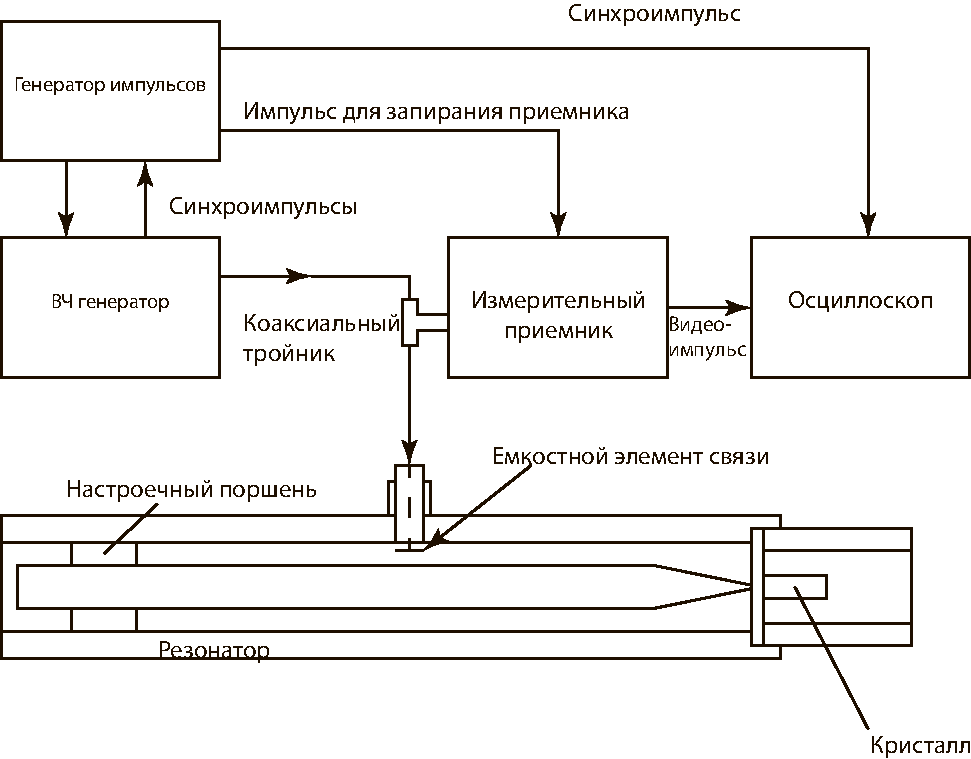
\includegraphics[width=0.5\textwidth]{scheme.png}
    \caption{Схема измерения параметров туннельного диода}
    \label{pic:scheme}
\end{figure}
	
Схема, используемая для получения статической характеристики диода, приведена на рисунке \ref{pic:scheme}. Ток измеряется миллиамперметром, включенным последовательно с диодом, а напряжение на диоде --- цифровым вольтметром. 
	
Плавно меняя сопротивление резистора $ R $ и тем самым повышая напряжение на диоде, получим вольт-амперную характеристику туннельного диода $I(U)$. Погрешность величин напряжения $U$ и тока $I$ оценим двумя единицами последнего разряда. Построим график зависимости $I(U)$. Он изображен на рисунке \ref{graf}. 
	
\begin{figure}[h]
    \includegraphics[scale=0.8]{graf.png}
    \caption{Измерение вольт-амперной характеристики $I(U)$ туннельного диода}
    \label{graf}
\end{figure}

Из графика определим искомые значения токов и напряжений:
	
\begin{itemize}
    \centering
    \item $ U_p = 0.04 \pm 0.02 $ В, $ I_p = 4.63 \pm 0.02 $ мА
    \item $ U_v = 0.32 \pm 0.02 $ В, $ I_v = 3.57 \pm 0.02 $ мА
    \item $ U_f = 0.47 \pm 0.02 $ В
\end{itemize} 

Примем $E_v = 0$. Тогда из выражения для $U_v \approx 2\mu e$ можно найти энергию Ферми $\mu_n \approx \mu_p$:

\[ \mu_n \approx \mu_p \approx eU_v/2 \approx 0.16 \text{ эВ} \]

Из выражения для напряжения $U_p \approx (\mu_n - E_\text{n max})/e$ получим энергию, соответствующую максимальной плотности распределения электронов $E_\text{n max}$:

\[ E_\text{n max} = \mu_n - eU_p \approx 0.12 \text{ эВ} \] 

\section{Вывод} 
В работе исследован принцип действия туннельного диода; мы наблюдали его вольт-амперную характеристику на осциллографе и затем измерили ее непосредственно, снимая зависимость тока от напряжения. 
	
По результатам измерений мы получили параметры диода, которые совпадают с грубой оценкой, полученной благодаря наблюдению на осциллографе.	
\end{document}
